\documentclass[conference]{IEEEtran}
\IEEEoverridecommandlockouts
% The preceding line is only needed to identify funding in the first footnote. If that is unneeded, please comment it out.
\usepackage{cite}
\usepackage{amsmath,amssymb,amsfonts}
\usepackage{algorithmic}
\usepackage{graphicx}
\usepackage{textcomp}
\usepackage{xcolor}
\usepackage{tabularx}
\usepackage{multirow}
\usepackage{graphics} % for pdf, bitmapped graphics files
\usepackage{subfig}
\usepackage{subcaption}
\usepackage{hyperref}
\usepackage{academicons}
\usepackage{xcolor}
\def\BibTeX{{\rm B\kern-.05em{\sc i\kern-.025em b}\kern-.08em
		T\kern-.1667em\lower.7ex\hbox{E}\kern-.125emX}}
% Gráficas en MATLAB
\usepackage{tikz, pgfplots}
% Color Enlace
\definecolor{colorEnlace}{RGB}{0, 0, 0}
\hypersetup{
	colorlinks=true,
	linkcolor=colorEnlace,
	citecolor=colorEnlace,
	urlcolor=colorEnlace,
	pdfauthor={Circuitos Electrónicos II},
	pdftitle={Introducción a LaTeX}
}
% Control 
\usepackage{amsmath}
\begin{document}
	
	\title{Acondicionamiento de señal de un sensor de humedad caso Raphanus sativus}
	\author{
		\IEEEauthorblockN{Ing. Willy Vargas Mateos}
		\IEEEauthorblockA{
			 Circuitos Electrónicos II\\
			Cusco, Perú\\
			willy.vargas@unsaac.edu.pe}
		\and
		\IEEEauthorblockN{Ruth Juana Espino Puma}
		\IEEEauthorblockA{
			Estudiante de Ingeniería Electrónica \\
			Cusco, Perú \\
			184657@unsaac.edu.pe}
		\and
		\IEEEauthorblockN{Davis Bremdow Salazar Roa}
		\IEEEauthorblockA{
			Estudiante de Ingeniería Electrónica \\
			Cusco, Perú \\
			200353@unsaac.edu.pe
		}
	}
	\maketitle
	\begin{abstract}This paper presents the design and implementation of a soil moisture monitoring system using the YL-69 sensor, aimed at optimizing water usage in agricultural applications. To enhance the accuracy and stability of the measurements, the sensor’s weak analog signal is conditioned using operational amplifiers (op-amps). A non-inverting amplifier is used to boost the signal, while a low-pass filter eliminates noise, enabling efficient processing by a Raspberry . The system controls automated irrigation by activating or deactivating water flow based on real-time soil moisture levels. This design not only improves irrigation management precision but also prevents overwatering, promoting healthy crop growth and supporting sustainable agricultural practices through the use of modern technologies like Raspberry.
		
	\end{abstract}
	
	\begin{IEEEkeywords}
		Sensor de humedad YL-69, Arduino UNO, Acondicionamiento de una señal
	\end{IEEEkeywords}
	
	% // ================== INTRODUCCIÓN ================== //
	\section{Introducción}
	La calidad del suelo es un factor determinante en el desarrollo de cultivos, ya que influye directamente en su crecimiento y productividad. En relación con la contaminación, esta puede definirse como la presencia de sustancias externas o de elementos en cantidades excesivas que alteran el equilibrio del suelo. Un ejemplo de esto es el exceso de agua, causado por un riego ineficiente, que puede generar efectos fisiológicos negativos para las plantas, como la asfixia radicular y la disminución de la absorción de nutrientes. En sistemas de agricultura controlada, este tipo de problemas puede deberse a una gestión inadecuada de los sensores de humedad del suelo, como el sensor YL-69.
	
	El sensor YL-69 es ampliamente utilizado en aplicaciones agrícolas para medir la humedad del suelo, pero su señal analógica débil y sensible al ruido requiere un adecuado acondicionamiento para garantizar lecturas precisas y estables. La integración de amplificadores operacionales (op-amps) en estos sistemas de monitoreo puede mejorar significativamente la precisión y estabilidad de los datos recogidos. Al amplificar la señal, filtrar el ruido y adaptar los niveles de voltaje, los op-amps permiten crear sistemas de riego más eficientes, evitando tanto el exceso como la falta de agua, y promoviendo un manejo óptimo del suelo en la agricultura de precisión.
	% // ================== OBJETIVOS ================== //
	\section{Objetivos}
	
	\begin{itemize}
		\item Acondicionamiento de la señal mediante la reducción del ruido
		\item Implementación de un sistema para la medición de humedad con la planta Raphanus sativus
	\end{itemize}
	% // ================== ESTUDIOS RELACIONADOS ================== //
	\section{Estudios Relacionados}
	
	En \cite{iotmonitoring} se describe un sistema de monitoreo de pH y humedad del suelo agrícola basado en tecnología de redes de sensores inalámbricos (IoT) el cual se enfoca en la importancia de la humedad para las plantas y la comparación de datos para medir el porcentaje de error entre las mediciones mediante la red inalámbrica obteniéndose para ello una diferencia del valor real del 1\%.
	
	Por otro lado \cite{chrysanthemum} se hace uso de un invernadero para monitorear el crecimiento de crisantemos mediante el control de humedad y un sistema de alarma cuando los niveles de tal parámetro se encontraban fuera del rango permitido, siendo además el enfoque principal el entorno adecuado para el crecimiento de los crisantemos a unas determinadas condiciones.
	
	En \cite{astromelia} se enfoca en el desarrollo de una red de sensores para el control de humedad para el cultivo de astromelias recuperando las mediciones obtenidas para su registro en una base de datos MySQL mediante una conexión inalambrica Wi-Fi para un monitoreo en tiempo real sobre el estado de la humedad en la tierra para luego realizar el procesamiento de los datos registrados para optimizar las variables ambientales.
	
	Finalmente en \cite{lowcosthumidity} se realzaron mediciones sobre el nivel de humedad del suelo para el proceso de compostaje de los desechos alimentarios en el cual se desarrollaron 2 modelos para la medición de la humedad del suelo, los cuales les permitieron obtener mediciones con un error del 5\% comprobando que el sensor YL-69 es un módulo electrónico adecuado para el monitoreo de humedad.
	
	% // ================== MARCO TEÓRICO ================== //
	\section{Marco Teórico} 
	
	
	% // ================== MATERIALES Y MÉTODOS ================== //
	\section{Materiales y métodos}
	\subsection{Sensor de humedad YL-69}
	Este sensor tiene la capacidad de medir la humedad del suelo. Aplicando una pequeña tensión entre los terminales del módulo YL-69 hace pasar una corriente que depende básicamente de la resistencia que se genera en el suelo y ésta depende mucho de la humedad. Por lo tanto al aumentar la humedad la corriente crece y al bajar la corriente disminuye.
	\begin{figure}
		\centering
		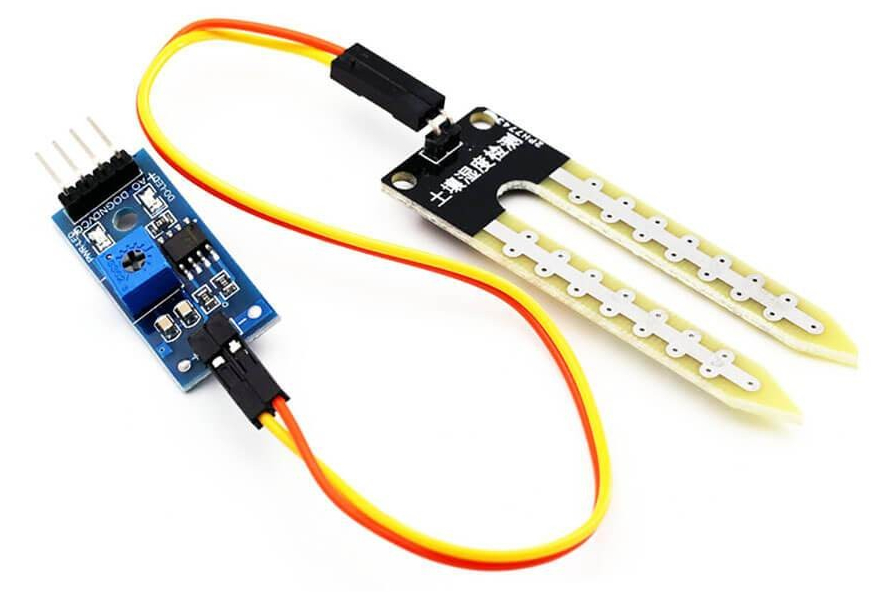
\includegraphics[width=0.5\textwidth]{media/[YL-69] YL-69 Soil Moisture Hygrometer Detection Humidity Sensor Module For arduino Development Board DIY .jpg}
		\caption{Sensor de Humedad YL-69}
		\label{fig:enter-label}
	\end{figure}
	\subsubsection{Características}
	\begin{itemize}
		\item Voltaje de operación(3.3v-5v)
		\item Modo de salida dual, salida digital y salida analógica más precisa.
		\item Dimensiones de sonda: 60mm/30mm (largo/ancho)
		\item Sensibilidad ajustable mediante potenciómetro digital.
		\item Indicadores led: alimentación (rojo) e indicador de salida de conmutación digital (verde).
		\item El módulo tiene un amplificador LM393
	\end{itemize}
	\subsubsection{Restricciones}
	\begin{itemize}
		\item Precisión limitada: No proporciona una medición altamente precisa de la humedad del suelo. 
		\item Corrosión: Las sondas están hechas de un material que puede corroerse con el tiempo debido al contacto continuo con la humedad del suelo.
		\item Interferencias en el suelo: Minerales, sales u otros elementos en el suelo pueden afectar las lecturas, causando imprecisiones.
		\item Alcance corto: Detecta humedad solo en el área inmediata alrededor de las sondas, lo que puede no representar correctamente el estado general del suelo
		\item Consumo de energía: Mantenerlo constantemente encendido puede resultar en un consumo de energía elevado
		\item Lecturas no calibradas: No tiene una calibración interna, por lo que las lecturas pueden variar entre diferentes sensores o entornos, necesitando ajustes adicionales.
	\end{itemize}
	
	\subsection{Arduino UNO}
	El Arduino UNO es una plataforma de hardware libre basada en un microcontrolador ATmega328P. Se utiliza en el desarrollo de proyectos electrónicos y educativos debido a su simplicidad y versatilidad. Posee 14 pines digitales de entrada/salida, 6 entradas analógicas, y una interfaz USB para conectarse a la computadora. Su principal ventaja es la facilidad para programar el microcontrolador mediante el lenguaje de programación Arduino, que se basa en C/C++. El Arduino UNO es ampliamente utilizado en prototipos de automatización, robótica y control de sistemas, permitiendo a los usuarios interactuar con sensores y actuadores de forma sencilla.
	
	\begin{figure}[h]
		\centering
		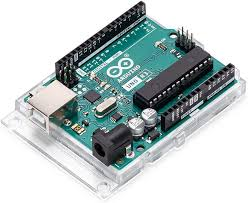
\includegraphics[width=0.4\textwidth]{media/arduino-uno.jpg}
		\caption{Arduino UNO}
		\label{fig:arduino-uno}
	\end{figure}
	
	\subsection{Filtros de ruido}
	Los filtros de ruido son dispositivos o algoritmos diseñados para eliminar o reducir el ruido no deseado en señales eléctricas, acústicas o digitales. Se clasifican en:
	
	\begin{itemize}
		\item Filtros pasivos: Utilizan componentes pasivos como resistencias, condensadores e inductores. Son simples y no requieren alimentación externa.
		\item Filtros activos: Incorporan amplificadores operacionales para mejorar la señal, permitiendo una mayor precisión.
		\item Filtros digitales: Procesan señales en el dominio digital mediante algoritmos. Son flexibles y se pueden adaptar para diferentes tipos de ruido. El objetivo principal de los filtros es mejorar la calidad de la señal útil, facilitando su interpretación o procesamiento posterior.
	\end{itemize}
	
	\begin{figure}[h]
		\centering
		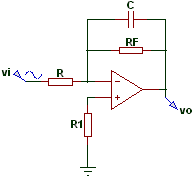
\includegraphics[width=0.3\textwidth]{media/filtro-pasa-bajos.png}
		\caption{Filtro pasabajos de primer orden}
		\label{fig:filtro-pasabajos}
	\end{figure}
	
	\subsection{Raphanus Sativus}
	El Raphanus sativus, comúnmente conocido como rábano, es una planta comestible perteneciente a la familia de las Brassicaceae. Se cultiva principalmente por su raíz comestible, la cual tiene un sabor picante característico. Esta planta es rica en vitaminas, minerales, y ha sido utilizada en medicina tradicional por sus propiedades digestivas y antioxidantes. Además, el rábano juega un rol importante en la agricultura como cultivo de rotación y mejora del suelo debido a su capacidad de aflojar la tierra y suprimir malezas.
	
	\begin{figure}[h]
		\centering
		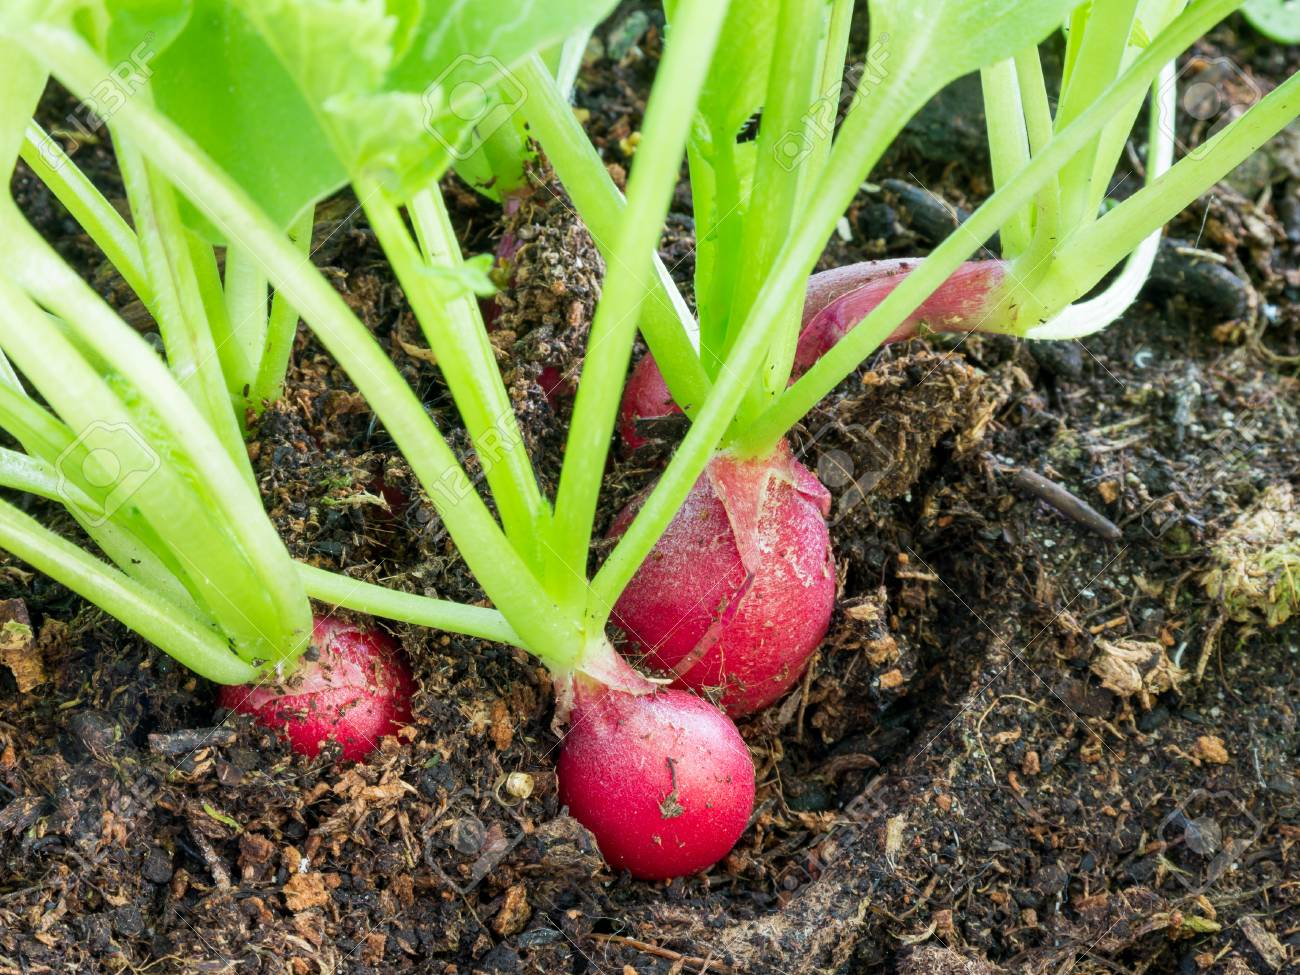
\includegraphics[width=0.4\textwidth]{media/raphanos.jpg}
		\caption{Raphanus sativus : Rabano}
		\label{fig:raphanus-sativus}
	\end{figure}
	
	
	% // ================== IMPLEMENTACIÓN ================== //
	\section{Implementación}
	
	\bibliographystyle{IEEEtran}
	\bibliography{biblio}
\end{document}